\documentclass[aspectratio=169, 11pt]{beamer}

% Packages
\usepackage[utf8]{inputenc}
\usepackage{amsmath, amssymb, amsfonts}
\usepackage{graphicx}
\usepackage{booktabs}
\usepackage{ragged2e}
\usepackage{minted}
\usepackage{xcolor}
\usepackage{tikz}
\usepackage{algorithm}
\usepackage{algorithmic}
\usepackage{listings}
\usepackage{tcolorbox}

\usetikzlibrary{arrows.meta,positioning,fit,shapes.symbols}
\usetikzlibrary{arrows,shapes}
\definecolor{LightGray}{gray}{0.975}
\definecolor{links}{HTML}{2A1B81}
\hypersetup{colorlinks,linkcolor=,urlcolor=blue}
\AtBeginEnvironment{minted}{%
    \renewcommand{\fcolorbox}[4][]{#4}
}

\title[Model Selection \& Regularization]{ML101 \\ Chapter 06: Linear Model Selection and Regularization}
\subtitle{An Introduction to Statistical Learning, ISLRv2}
\author{James, Witten, Hastie \& Tibshirani}
\date{\today}

% Remove navigation symbols
\setbeamertemplate{navigation symbols}{}

\defbeamertemplate*{footline}{shadow theme}{
    \leavevmode
    \hbox{
        \begin{beamercolorbox}[
                wd =        0.33\paperwidth,
                ht =        2.5ex,
                dp =        1.125ex,
                leftskip =  0.3cm plus1fil,
                rightskip = 0.3cm
            ]{author in head/foot}
            \flushleft ML101
        \end{beamercolorbox}
        \begin{beamercolorbox}[
                wd =        0.33\paperwidth,
                ht =        2.5ex,
                dp =        1.125ex,
                leftskip =  0.3cm plus1fil,
                rightskip = 0.3cm
            ]{author in head/foot}
            \insertshorttitle
        \end{beamercolorbox}
        \begin{beamercolorbox}[
                wd =        0.33\paperwidth,
                ht =        2.5ex,
                dp =        1.125ex,
                leftskip =  0.3cm plus1fil,
                rightskip = 0.3cm
            ]{title in head/foot}
            \hfill \insertframenumber\,/\,\inserttotalframenumber%
        \end{beamercolorbox}
    }
}

\AtBeginSection[]
{
     \begin{frame}<beamer>
     \frametitle{Plan}
     \tableofcontents[currentsection]
     \end{frame}
}

\usefonttheme{serif}

\newcommand\Wider[2][18mm]{%
    \makebox[\linewidth][c]{%
        \begin{minipage}{\dimexpr\textwidth+#1\relax}
            \raggedright#2
        \end{minipage}%
    }%
}
\newcommand\userinput[1]{\textbf{#1}}

\begin{document}

\frame{\titlepage}

\begin{frame}{An Introduction to Statistical Learning with Applications in R}{a.k.a. ISLR}
    \centering
    
\includegraphics[height=0.7\textheight]{figures/book_cover} \\
    \vspace{4mm}
    {
        \tiny
        Content has been extracted from \textit{An Introduction to Statistical Learning with Applications in R}, Second Edition, by James, Witten, Hastie \& Tibshirani. Springer. 2023.\\
        Visit \url{https://www.statlearning.com/}.\\
    }
\end{frame}

\begin{frame}{In Praise of Linear Models!}
    \begin{itemize}
        \item Recall the standard linear regression model:
        \[
            Y = \beta_0 + \beta_1 X_1 + \dots + \beta_p X_p + \epsilon
        \]
        \item \textbf{Why stick with linear models?}
        \begin{itemize}
            \item High degree of \textbf{interpretability}.
            \item Often competitive in \textbf{predictive performance} compared to non-linear black-box methods.
            \item Computationally straightforward and well-understood theoretical foundations.
        \end{itemize}
        \vspace{0.5em}
        \item In this lecture, we improve ordinary least squares (OLS) by considering alternative fitting procedures to overcome key limitations.
    \end{itemize}
\end{frame}

\begin{frame}{Why Consider Alternatives to Least Squares?}
    \begin{columns}[T]
        \begin{column}{0.48\textwidth}
            \begin{block}{1. Prediction Accuracy}
                \begin{itemize}
                    \item When $n \gg p$, OLS estimates tend to have low variance.
                    \item If $n$ is not much larger than $p$, OLS fit can suffer from \textbf{high variability}, leading to overfitting.
                    \item If $p > n$, OLS has \textbf{no unique solution} (variance is infinite).
                    \item Constraining or shrinking coefficients trades a tiny increase in bias for a substantial drop in variance.
                \end{itemize}
            \end{block}
        \end{column}

        \begin{column}{0.48\textwidth}
            \begin{block}{2. Model Interpretability}
                \begin{itemize}
                    \item Multiple regression models often include variables that are unrelated to the response.
                    \item OLS rarely sets coefficient estimates exactly to zero ($\hat{\beta}_j \neq 0$).
                    \item Retaining irrelevant variables introduces clutter and reduces interpretability.
                    \item We desire automated methods for \textbf{feature selection} (sparsity).
                \end{itemize}
            \end{block}
        \end{column}
    \end{columns}
\end{frame}

\begin{frame}{Three Classes of Methods}
    \begin{enumerate}
        \item \textbf{Subset Selection:}
        \begin{itemize}
            \item Identify a subset of the $p$ predictors believed to be related to the response.
            \item Fit a model using standard least squares on the reduced set of variables.
        \end{itemize}
        \vspace{0.5em}
        \item \textbf{Shrinkage (Regularization):}
        \begin{itemize}
            \item Fit a model involving all $p$ predictors, but shrink estimated coefficients towards zero relative to OLS.
            \item Reduces variance significantly; specific forms (e.g., Lasso) also perform variable selection.
        \end{itemize}
        \vspace{0.5em}
        \item \textbf{Dimension Reduction:}
        \begin{itemize}
            \item Project the $p$ predictors into an $M$-dimensional subspace ($M < p$) using linear combinations.
            \item Fit a least squares regression model using these $M$ new projected features.
        \end{itemize}
    \end{enumerate}
\end{frame}

\section{Subset Selection}

\begin{frame}{Best Subset Selection}
    \begin{block}{Algorithm: Best Subset Selection}
    \begin{enumerate}
        \item Let $\mathcal{M}_0$ denote the \textbf{null model}, which contains no predictors (predicts sample mean $\bar{y}$).
        \item For $k = 1, 2, \dots, p$:
        \begin{enumerate}[(a)]
            \item Fit all $\binom{p}{k} = \frac{p!}{k!(p-k)!}$ models containing exactly $k$ predictors.
            \item Pick the best among these $\binom{p}{k}$ models, called $\mathcal{M}_k$ (lowest RSS or highest $R^2$).
        \end{enumerate}
        \item Select a single best model from among $\mathcal{M}_0, \mathcal{M}_1, \dots, \mathcal{M}_p$ using cross-validated prediction error, $C_p$ (AIC), BIC, or adjusted $R^2$.
    \end{enumerate}
    \end{block}
    \begin{itemize}
        \item \textbf{Crucial distinction:} Step 2 uses training RSS/$R^2$ to compare models of the \emph{same size}. Step 3 uses test-error estimates to compare models of \emph{different sizes}.
    \end{itemize}
\end{frame}

\begin{frame}{Best Subset Selection on Credit Data}
    \centering
    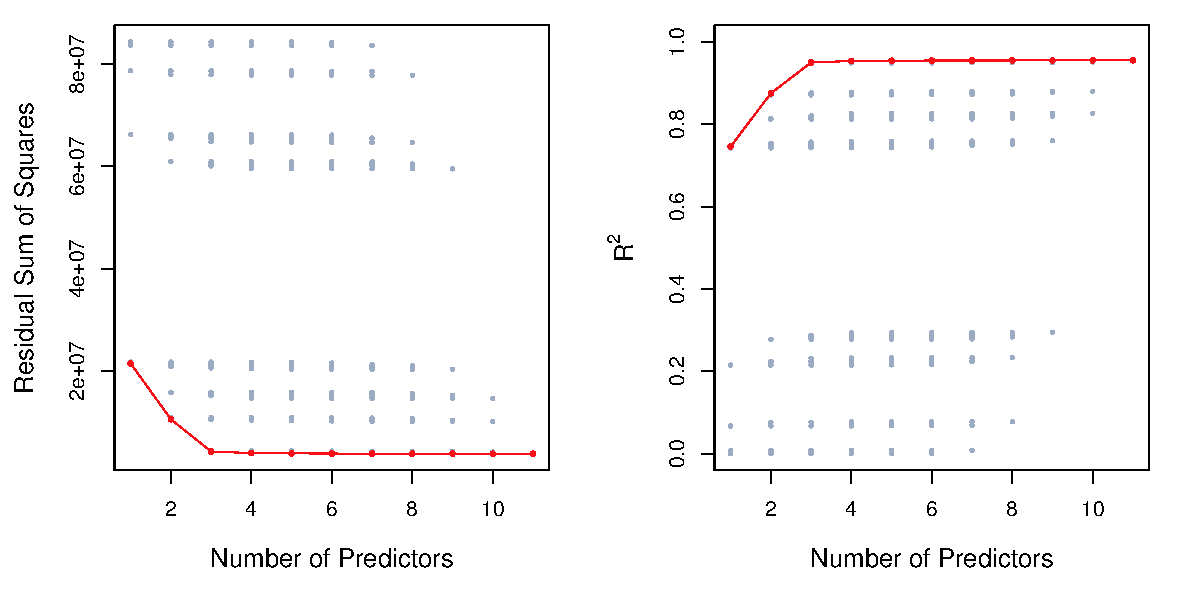
\includegraphics[width=0.8\textwidth]{figures/6_1}
    \begin{itemize}
        \footnotesize
        \item \textbf{Left Panel:} Residual Sum of Squares (RSS) for all possible subset models of the \texttt{Credit} data. As subset size $k$ increases, training RSS decreases monotonically.
        \item \textbf{Right Panel:} Corresponding $R^2$ values increasing monotonically to 1.
        \item \textbf{Red Frontier:} Highlights the best model $\mathcal{M}_k$ for each subset size $k$.
    \end{itemize}
\end{frame}

\begin{frame}{Forward Stepwise Selection}
    \begin{itemize}
        \item Best subset selection is computationally intractable for large $p$ (searches $2^p$ models; if $p=40$, $2^{40} \approx 1.1 \times 10^{12}$ models).
        \item \textbf{Forward stepwise selection} offers a greedy, computationally efficient alternative:
    \end{itemize}
    \begin{block}{Algorithm: Forward Stepwise Selection}
    \begin{enumerate}
        \item Let $\mathcal{M}_0$ denote the null model.
        \item For $k = 0, 1, \dots, p-1$:
        \begin{enumerate}[(a)]
            \item Consider all $p - k$ models that augment $\mathcal{M}_k$ with one additional predictor.
            \item Choose the best among these $p - k$ models (smallest RSS / highest $R^2$), and call it $\mathcal{M}_{k+1}$.
        \end{enumerate}
        \item Select the overall best model among $\mathcal{M}_0, \dots, \mathcal{M}_p$ via CV, $C_p$, AIC, BIC, or adjusted $R^2$.
    \end{enumerate}
    \end{block}
    \begin{itemize}
        \item Fits only $1 + \sum_{k=0}^{p-1}(p-k) = 1 + \frac{p(p+1)}{2}$ models (for $p=20$: 211 vs. 1,048,576).
    \end{itemize}
\end{frame}

\begin{frame}{Backward Stepwise Selection}
    \begin{block}{Algorithm: Backward Stepwise Selection}
    \begin{enumerate}
        \item Let $\mathcal{M}_p$ denote the \textbf{full model}, which contains all $p$ predictors.
        \item For $k = p, p-1, \dots, 1$:
        \begin{enumerate}[(a)]
            \item Consider all $k$ models that contain all but one predictor in $\mathcal{M}_k$ ($k - 1$ predictors).
            \item Choose the best among these $k$ models (smallest RSS / highest $R^2$), and call it $\mathcal{M}_{k-1}$.
        \end{enumerate}
        \item Select the single best model among $\mathcal{M}_0, \dots, \mathcal{M}_p$ using CV, $C_p$, AIC, BIC, or adjusted $R^2$.
    \end{enumerate}
    \end{block}
    \begin{itemize}
        \item Like forward stepwise, considers only $1 + p(p+1)/2$ models.
        \item \textbf{Constraint:} Requires $n > p$ so that the initial full model $\mathcal{M}_p$ can be fit by least squares.
        \item In contrast, forward stepwise can be used when $n < p$ (constructing submodels up to $\mathcal{M}_{n-1}$).
    \end{itemize}
\end{frame}

\begin{frame}{Credit Data: Subset Comparison}
    \begin{table}
        \centering
        \small
        \begin{tabular}{c l l}
            \toprule
            \textbf{\# Variables} & \textbf{Best Subset Selection} & \textbf{Forward Stepwise Selection} \\
            \midrule
            \textbf{1} & \texttt{rating} & \texttt{rating} \\
            \textbf{2} & \texttt{rating}, \texttt{income} & \texttt{rating}, \texttt{income} \\
            \textbf{3} & \texttt{rating}, \texttt{income}, \texttt{student} & \texttt{rating}, \texttt{income}, \texttt{student} \\
            \textbf{4} & \texttt{cards}, \texttt{income}, \texttt{student}, \texttt{limit} & \texttt{rating}, \texttt{income}, \texttt{student}, \texttt{limit} \\
            \bottomrule
        \end{tabular}
    \end{table}
    \begin{itemize}
        \item For $k=1, 2, 3$, both methods identify the exact same predictor set.
        \item At $k=4$, best subset drops \texttt{rating} in favor of \texttt{cards} and \texttt{limit}.
        \item Forward stepwise is \textbf{nested} ($\mathcal{M}_k \subset \mathcal{M}_{k+1}$); it cannot drop \texttt{rating} once added.
    \end{itemize}
\end{frame}

\begin{frame}{Choosing the Optimal Model: Adjusted Criteria}
    To compare models with different numbers of predictors $d$, we adjust training RSS:
    \begin{columns}[T]
        \begin{column}{0.48\textwidth}
            \begin{block}{Mallows' $C_p$ and AIC}
                \[
                    C_p = \frac{1}{n}\left(\text{RSS} + 2d\hat{\sigma}^2\right)
                \]
                \[
                    \text{AIC} = \frac{1}{n\hat{\sigma}^2}\left(\text{RSS} + 2d\hat{\sigma}^2\right)
                \]
                \begin{itemize}
                    \small
                    \item $\hat{\sigma}^2$ is an unbiased estimate of error variance $\sigma^2$ from the full model.
                    \item Penalizes model size by adding $2d\hat{\sigma}^2$.
                \end{itemize}
            \end{block}
        \end{column}

        \begin{column}{0.48\textwidth}
            \begin{block}{BIC and Adjusted $R^2$}
                \[
                    \text{BIC} = \frac{1}{n}\left(\text{RSS} + \log(n)d\hat{\sigma}^2\right)
                \]
                \[
                    \text{Adjusted } R^2 = 1 - \frac{\text{RSS}/(n-d-1)}{\text{TSS}/(n-1)}
                \]
                \begin{itemize}
                    \small
                    \item For $n > 7$, $\log(n) > 2$; hence \textbf{BIC penalizes larger models more heavily} than $C_p$.
                    \item For $C_p$, AIC, BIC: \textbf{smaller is better}.
                    \item For Adjusted $R^2$: \textbf{larger is better}.
                \end{itemize}
            \end{block}
        \end{column}
    \end{columns}
\end{frame}

\begin{frame}{Model Selection: Adjusted Criteria vs. Validation/CV}
    \centering
    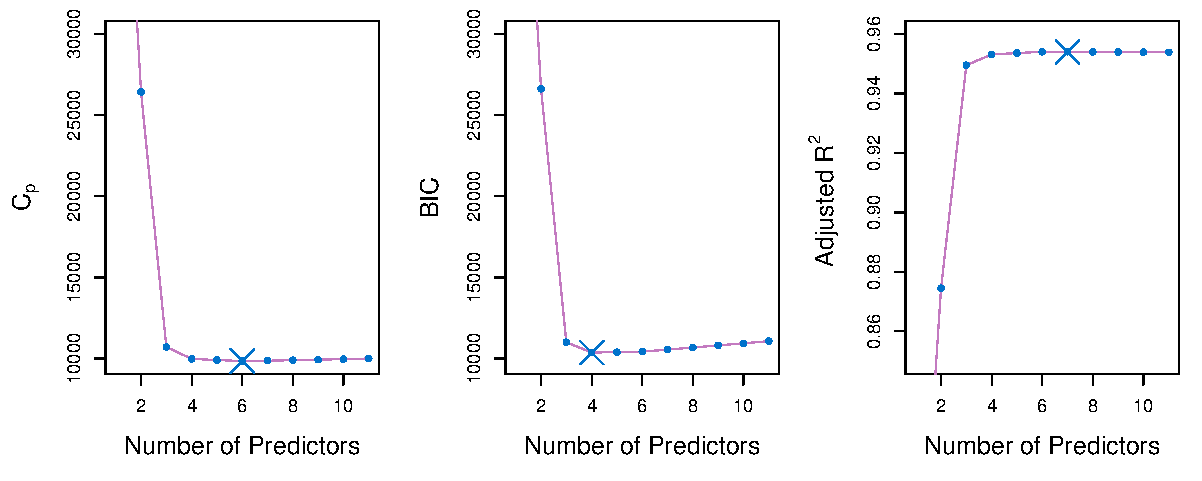
\includegraphics[width=0.9\textwidth]{figures/6_2}
    \begin{itemize}
        \footnotesize
        \item Plots of $C_p$, BIC, and Adjusted $R^2$ (top row) alongside Validation Set and 10-Fold Cross-Validation error curves (bottom row) for \texttt{Credit} data models.
        \item BIC chooses a parsimonious 4-variable model (\texttt{income}, \texttt{limit}, \texttt{cards}, \texttt{student}), while $C_p$ and Adjusted $R^2$ choose 6 variables.
    \end{itemize}
\end{frame}

\begin{frame}{Model Selection: Adjusted Criteria vs. Validation/CV --continued}
    \centering
    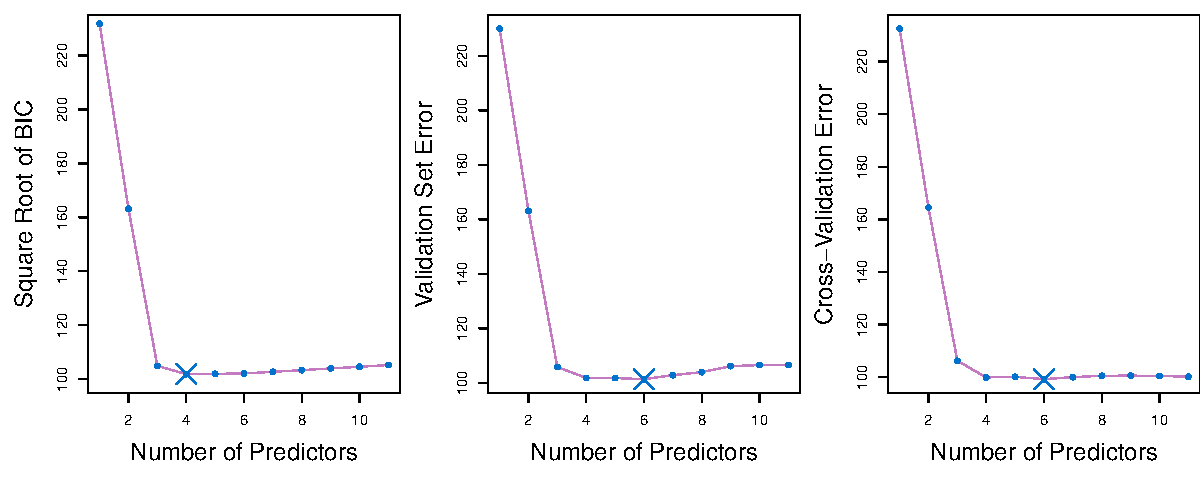
\includegraphics[width=0.9\textwidth]{figures/6_3}
    \begin{itemize}
        \footnotesize
        \item Cross-validation curve is flat between 4 and 11 variables, showing that extra variables add little test predictive power.
    \end{itemize}
\end{frame}

\begin{frame}{The One-Standard-Error Rule}
    \begin{block}{Definition: One-Standard-Error Rule}
        When comparing a set of models via cross-validation, calculate the standard error of the estimated test MSE for each model size. 
        \begin{itemize}
            \item Identify the model with the minimum cross-validation error.
            \item Select the \textbf{simplest (most parsimonious) model} whose CV error is within \textbf{1 standard error} of the minimum.
        \end{itemize}
    \end{block}
    \begin{itemize}
        \item \textbf{Rationale:} Acknowledges that differences in CV error within $1\,\text{SE}$ are likely due to random sampling variability.
        \item Adheres to Occam's razor: favor simpler, more interpretable models when empirical performance is statistically indistinguishable.
    \end{itemize}
\end{frame}

\section{Shrinkage Methods}

\begin{frame}{Ridge Regression}
    \begin{itemize}
        \item Standard OLS minimizes $\text{RSS} = \sum_{i=1}^n \left(y_i - \beta_0 - \sum_{j=1}^p \beta_j x_{ij}\right)^2$.
        \item \textbf{Ridge regression} minimizes a penalized objective:
        \[
            \hat{\beta}^R_\lambda = \arg\min_{\beta} \left\{ \sum_{i=1}^n \left( y_i - \beta_0 - \sum_{j=1}^p \beta_j x_{ij} \right)^2 + \lambda \sum_{j=1}^p \beta_j^2 \right\} = \arg\min_{\beta} \left\{ \text{RSS} + \lambda \|\beta\|_2^2 \right\}
        \]
        \item $\lambda \ge 0$ is a \textbf{tuning parameter}:
        \begin{itemize}
            \item When $\lambda = 0$: penalty has no effect $\implies \hat{\beta}^R_0 = \hat{\beta}^{\text{OLS}}$.
            \item As $\lambda \to \infty$: shrinkage penalty dominates $\implies \hat{\beta}^R_\lambda \to 0$.
        \end{itemize}
        \item The intercept $\beta_0$ is \emph{not} penalized (estimated simply as $\bar{y}$ when predictors are centered).
        \item Uses the squared $\ell_2$ penalty: $\|\beta\|_2^2 = \sum_{j=1}^p \beta_j^2$.
    \end{itemize}
\end{frame}

\begin{frame}{Ridge Regression: Coefficient Profiles on Credit Data}
    \centering
    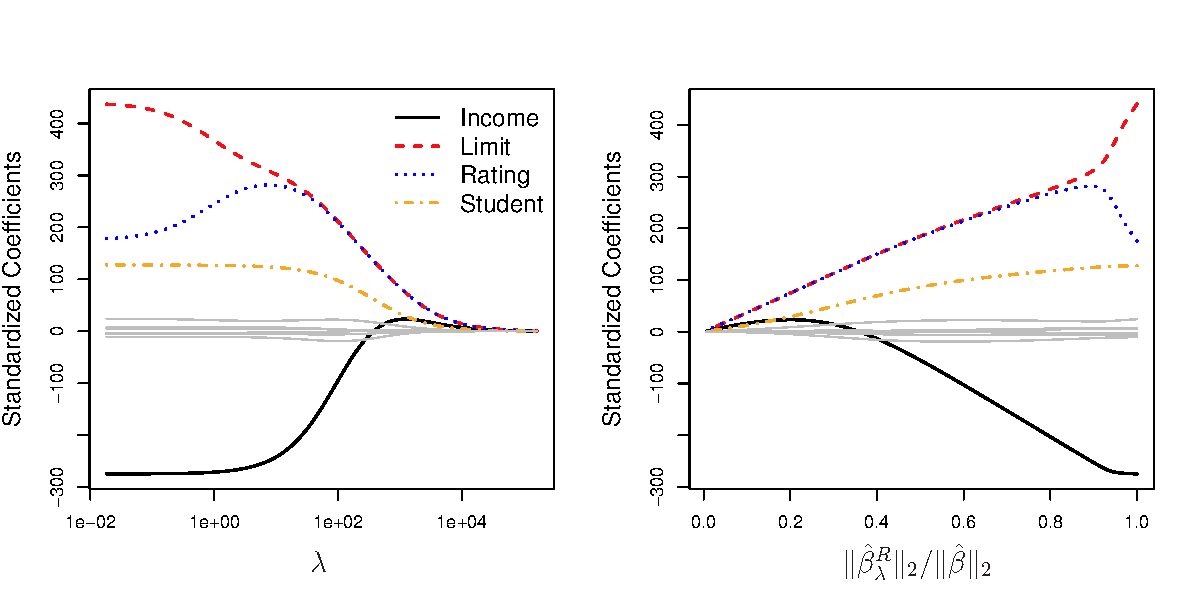
\includegraphics[width=0.8\textwidth]{figures/6_4}
    \begin{itemize}
        \footnotesize
        \item \textbf{Left Panel:} Standardized ridge regression coefficients for \texttt{Credit} predictors plotted against $\lambda$. As $\lambda$ increases, all coefficients shrink continuously towards zero.
        \item \textbf{Right Panel:} The same coefficients plotted as a function of $\|\hat{\beta}^R_\lambda\|_2 / \|\hat{\beta}^{\text{OLS}}\|_2$ (amount of shrinkage relative to OLS).
        \item Notice that \texttt{income}, \texttt{limit}, \texttt{rating}, and \texttt{student} remain the largest throughout.
    \end{itemize}
\end{frame}

\begin{frame}{Ridge Regression: Scaling of Predictors}
    \begin{itemize}
        \item OLS coefficient estimates are \textbf{scale equivariant}: multiplying $X_j$ by a constant $c$ simply scales $\hat{\beta}_j$ by $1/c$, leaving $X_j \hat{\beta}_j$ unchanged.
        \item In contrast, the ridge penalty $\lambda \sum \beta_j^2$ is \textbf{sensitive to predictor scaling}!
        \item A variable measured in dollars will have much smaller coefficients (and hence smaller penalty) than the same variable measured in thousands of dollars.
    \end{itemize}
    \begin{block}{Standardization Formula}
        Before applying ridge regression, standardizing all predictors to unit variance is essential:
        \[
            \tilde{x}_{ij} = \frac{x_{ij}}{\sqrt{\frac{1}{n} \sum_{i=1}^n (x_{ij} - \bar{x}_j)^2}}
        \]
    \end{block}
\end{frame}

\begin{frame}{Why Does Ridge Regression Improve Over OLS?}
    \centering
    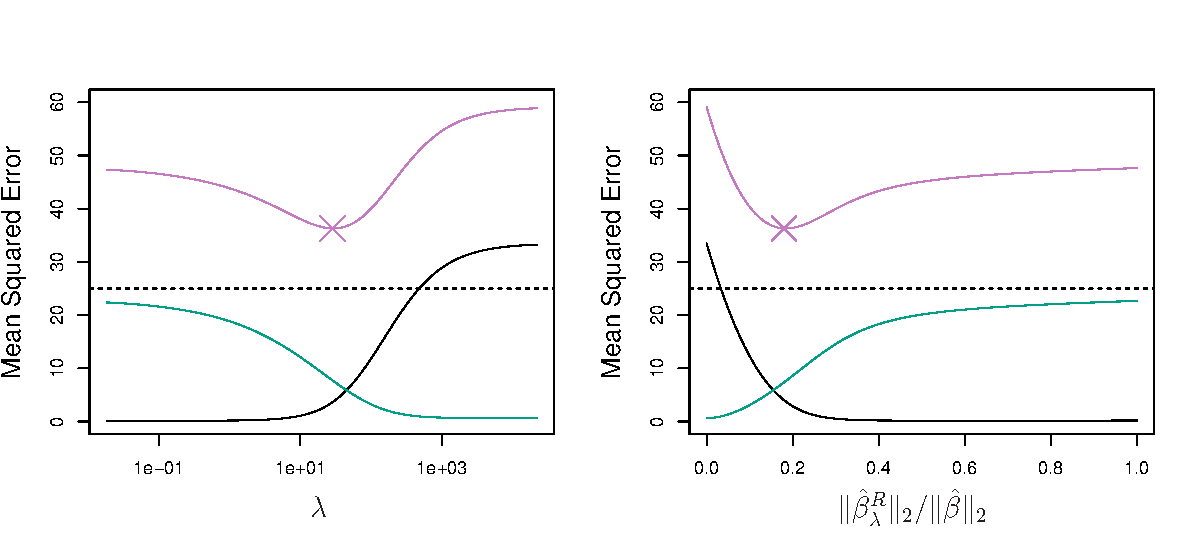
\includegraphics[width=0.8\textwidth]{figures/6_5}
    \begin{itemize}
        \footnotesize
        \item Simulation setting with $p = 45$ predictors and $n = 50$ observations.
        \item \textbf{Variance (green curve):} Extremely high at $\lambda = 0$ (OLS), but drops dramatically as $\lambda$ increases.
        \item \textbf{Squared Bias (black curve):} Zero at $\lambda = 0$, increases slowly at first, then climbs rapidly.
        \item \textbf{Test MSE (purple curve):} Exhibits a clear U-shape, achieving a minimum at an intermediate value of $\lambda \approx 30$.
    \end{itemize}
\end{frame}

\begin{frame}{The Lasso}
    \begin{itemize}
        \item \textbf{Disadvantage of Ridge:} It will shrink all coefficients close to zero, but \emph{never sets any coefficient exactly to zero} (unless $\lambda = \infty$).
        \item \textbf{The Lasso} replaces the $\ell_2$ penalty with an $\ell_1$ penalty:
    \end{itemize}
    $$
        \hat{\beta}^L_\lambda = \arg\min_{\beta} \left\{ \sum_{i=1}^n \left( y_i - \beta_0 - \sum_{j=1}^p \beta_j x_{ij} \right)^2 + \lambda \sum_{j=1}^p |\beta_j| \right\} = \arg\min_{\beta} \left\{ \text{RSS} + \lambda \|\beta\|_1 \right\}
    $$
    \begin{itemize}
        \item $\|\beta\|_1 = \sum_{j=1}^p |\beta_j|$ is the $\ell_1$ norm.
        \item The $\ell_1$ penalty forces some coefficients to be \textbf{identically zero} when $\lambda$ is sufficiently large.
        \item Hence, Lasso yields \textbf{sparse models} and performs automatic variable selection!
    \end{itemize}
\end{frame}

\begin{frame}{Example: Credit Dataset (Lasso)}
    \centering
    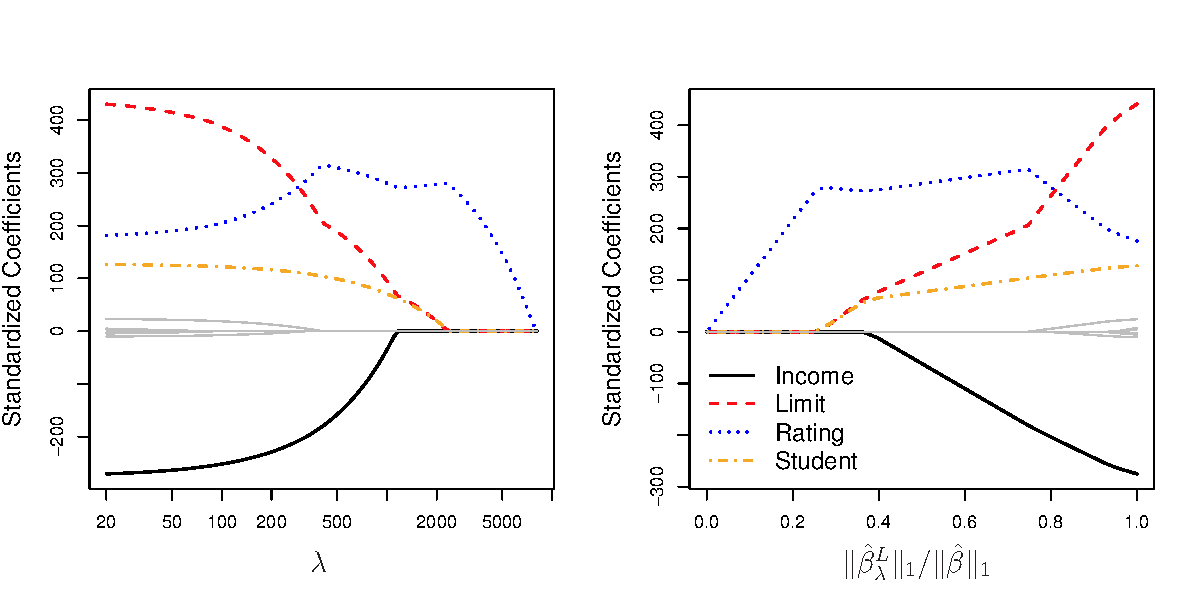
\includegraphics[width=0.9\textwidth]{figures/6_6}
    \begin{itemize}
        \footnotesize
        \item \textbf{Left Panel:} Standardized Lasso coefficients plotted against $\lambda$. For large $\lambda$, all coefficients are 0. As $\lambda$ decreases, \texttt{rating} enters first, followed by \texttt{student}, \texttt{limit}, and \texttt{income}.
        \item \textbf{Right Panel:} Lasso coefficients plotted against $\|\hat{\beta}^L_\lambda\|_1 / \|\hat{\beta}^{\text{OLS}}\|_1$. Clear variable entry points demonstrate step-by-step feature inclusion.
    \end{itemize}

\end{frame}

\begin{frame}{Budget Constraint Formulations}
    The Lasso and Ridge problems can be equivalently formulated as constrained optimizations:
    \begin{columns}[T]
        \begin{column}{0.48\textwidth}
            \begin{block}{Lasso Optimization ($\ell_1$ Budget)}
                \[
                    \min_{\beta} \text{RSS} \quad \text{subject to} \quad \sum_{j=1}^p |\beta_j| \le s
                \]
            \end{block}
        \end{column}

        \begin{column}{0.48\textwidth}
            \begin{block}{Ridge Optimization ($\ell_2$ Budget)}
                \[
                    \min_{\beta} \text{RSS} \quad \text{subject to} \quad \sum_{j=1}^p \beta_j^2 \le s
                \]
            \end{block}
        \end{column}
    \end{columns}
    \vspace{0.5em}
    \begin{itemize}
        \item For every $\lambda$, there corresponds a budget $s \ge 0$.
        \item If $s$ is very large, the budget constraint is non-binding, yielding the unconstrained OLS solution.
        \item If $s$ is small, the coefficients are constrained to lie strictly within the budget region.
    \end{itemize}
\end{frame}

\begin{frame}{The Variable Selection Property of the Lasso}
    \centering
    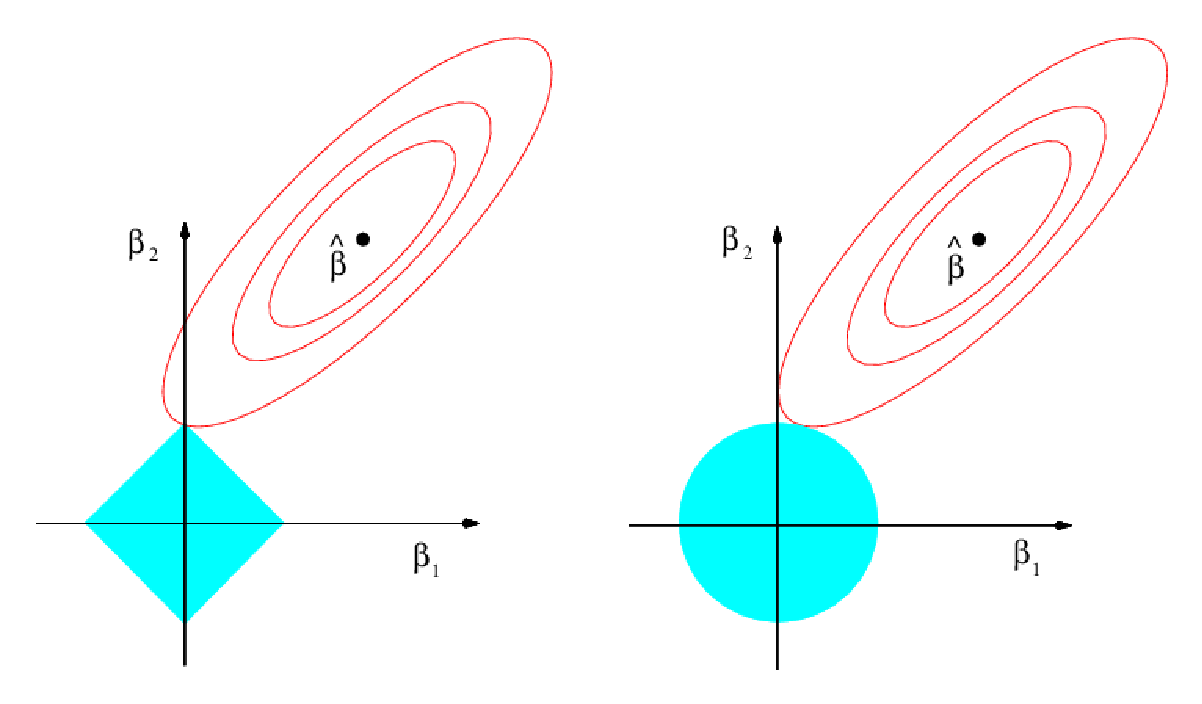
\includegraphics[width=0.7\textwidth]{figures/6_7}
    \vspace{-3mm}
    \begin{itemize}
        \footnotesize
        \item \textbf{Lasso (Left):} The constraint region is a diamond ($|\beta_1| + |\beta_2| \le s$) with sharp corners on the coordinate axes. The elliptical RSS contours frequently contact the diamond at a corner, forcing $\beta_1 = 0$.
        \item \textbf{Ridge (Right):} The constraint region is a circle ($\beta_1^2 + \beta_2^2 \le s$) with no corners. Contact points almost never lie on the axes, so both $\beta_1, \beta_2 \neq 0$.
    \end{itemize}
\end{frame}

\begin{frame}{Comparing Lasso and Ridge Regression}
    \centering
    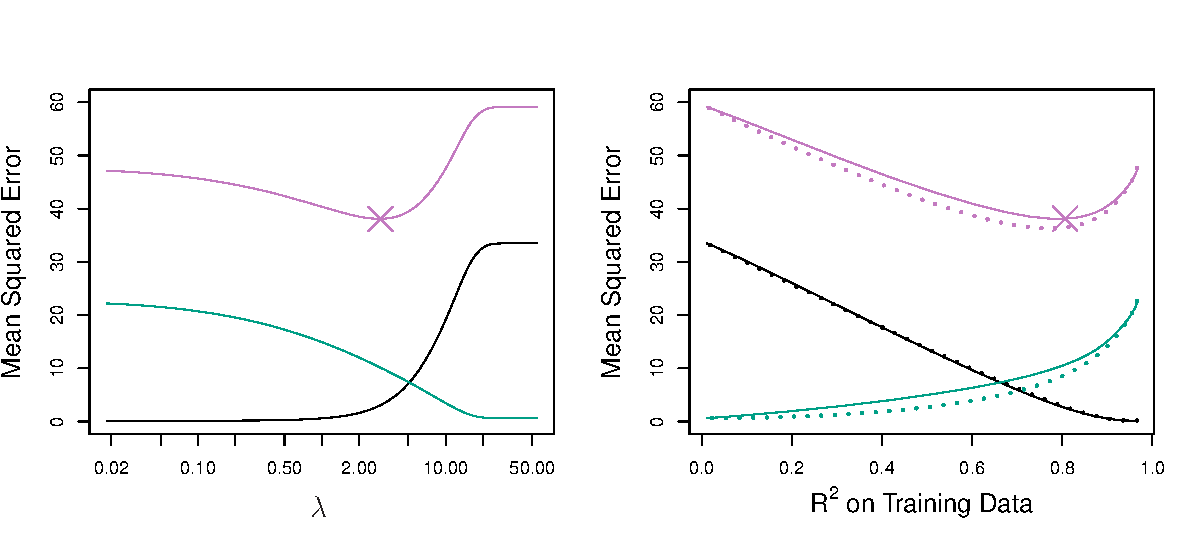
\includegraphics[width=0.9\textwidth]{figures/6_8}
    \begin{itemize}
        \footnotesize
        \item \textbf{Left}: Plots of squared bias (black), variance (green), and test MSE (purple) for the lasso on simulated data set of Slide 32.
        \item \textbf{Right}: Comparison of squared bias, variance and test \textit{MSE} between lasso (solid) and ridge (dashed). Both are plotted against their $R^2$ on the training data, as a common form of indexing. The crosses in both plots indicate the lasso model for which the \textit{MSE} is smallest.
    \end{itemize}
\end{frame}

\begin{frame}{Comparing Lasso and Ridge Regression}
    \centering
    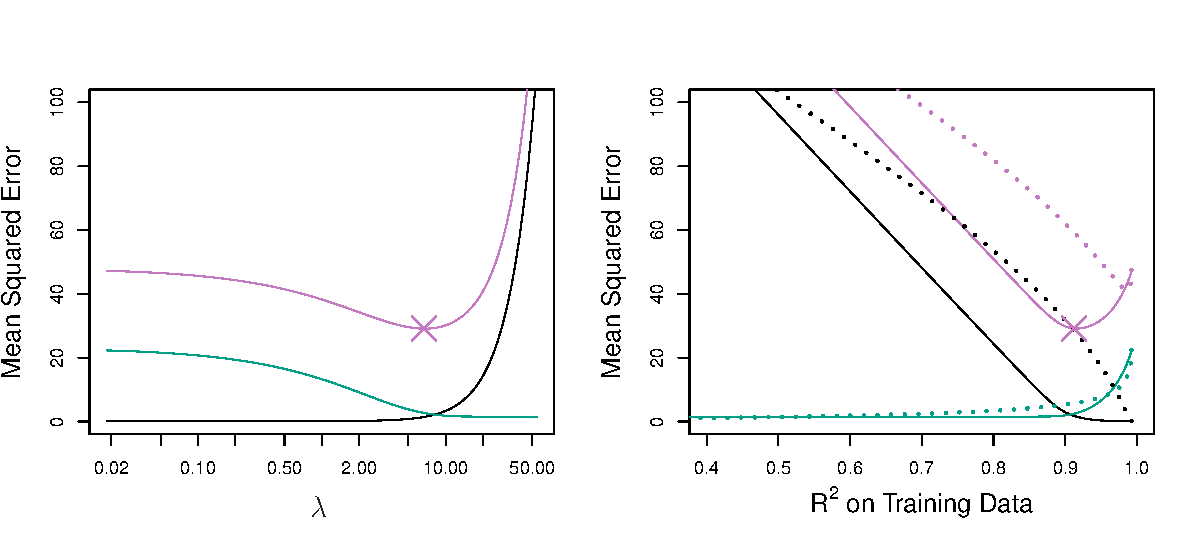
\includegraphics[width=0.9\textwidth]{figures/6_9}
    \begin{itemize}
        \footnotesize
        \item \textbf{Left}: Plots of squared bias (black), variance (green), and test \textit{MSE} (purple) for the lasso. The simulated data is similar to that in Slide 38, except that now only two predictors are related to the response.
        \item \textbf{Right}: Comparison of squared bias, variance and test \textit{MSE} between lasso (solid) and ridge (dashed). Both are plotted against their R2 on the training data, as a common form of indexing. The crosses in both plots indicate the lasso model for which the \textit{MSE} is smallest.
    \end{itemize}
\end{frame}

\begin{frame}{Comparing Lasso and Ridge Regression --continued}
    \begin{itemize}
        \item \textbf{Dense Setting (All 45 predictors non-zero):} Ridge regression slightly outperforms Lasso in test MSE because shrinking all variables together matches the underlying truth.
        \item \textbf{Sparse Setting (Only 2 of 45 predictors non-zero):} Lasso significantly outperforms Ridge because it successfully zeros out the 43 noise variables, drastically cutting variance.
    \end{itemize}
\end{frame}

\begin{frame}{Conclusions}
    \begin{itemize}
        \item These two examples illustrate that neither ridge regression nor the lasso will universally dominate the other.
        \item In general, one might expect the lasso to perform better when the response is a function of only a relatively small number of predictors.
        \item However, the number of predictors that is related to the response is never known \textbf{a priori} for real data sets.
        \item A technique such as cross-validation can be used in order to determine which approach is better on a particular data set.
    \end{itemize}
\end{frame}

\begin{frame}{Selecting the Tuning Parameter for Ridge Regression and Lasso}
    \begin{itemize}
        \item As for subset selection, for ridge regression and lasso we require a method to determine which of the models under consideration is best.
        \item That is, we require a method selecting a value for the tuning parameter $\lambda$ or equivalently, the value of the constraint $s$.
        \item \textbf{Cross-validation} provides a simple way to tackle this problem. We choose a grid of $\lambda$ values, and compute the cross-validation error rate for each value of $\lambda$.
        \item We then select the tuning parameter value for which the cross-validation error is smallest.
        \item Finally, the model is re-fit using all of the available observations and the selected value of the tuning parameter.
    \end{itemize}
\end{frame}

% \begin{frame}{Special Case: Orthogonal Predictors ($n = p, \mathbf{X} = \mathbf{I}$)}
%     When $n=p$ and $\mathbf{X}$ is orthonormal (with no intercept), OLS gives $\hat{\beta}_j = y_j$.
%     \begin{columns}[T]
%         \begin{column}{0.48\textwidth}
%             \begin{block}{Ridge: Proportional Shrinkage}
%                 \[
%                     \hat{\beta}^R_j = \frac{y_j}{1 + \lambda}
%                 \]
%                 \begin{itemize}
%                     \item Every coefficient is scaled down by a constant factor $\frac{1}{1+\lambda}$.
%                     \item Non-zero estimates remain non-zero.
%                 \end{itemize}
%             \end{block}
%         \end{column}
%
%         \begin{column}{0.48\textwidth}
%             \begin{block}{Lasso: Soft-Thresholding}
%                 \[
%                     \hat{\beta}^L_j = \begin{cases}
%                         y_j - \lambda/2 & \text{if } y_j > \lambda/2 \\
%                         y_j + \lambda/2 & \text{if } y_j < -\lambda/2 \\
%                         0 & \text{if } |y_j| \le \lambda/2
%                     \end{cases}
%                 \]
%                 \begin{itemize}
%                     \item Shrinks coefficients toward 0 by constant amount $\lambda/2$.
%                     \item Exactly zeros out coefficients with $|y_j| \le \lambda/2$.
%                 \end{itemize}
%             \end{block}
%         \end{column}
%     \end{columns}
% \end{frame}
%
% \begin{frame}{Bayesian Interpretation of Ridge and Lasso}
%     Assume $Y = \mathbf{X}\beta + \epsilon$ with Gaussian noise $\epsilon \sim \mathcal{N}(0, \sigma^2 \mathbf{I})$, and prior $p(\beta) = \prod_{j=1}^p g(\beta_j)$:
%     \begin{itemize}
%         \item \textbf{Gaussian Prior (Ridge):} $g(\beta_j) = \frac{1}{\sqrt{2\pi\sigma_0^2}}\exp\left(-\frac{\beta_j^2}{2\sigma_0^2}\right)$
%         \begin{itemize}
%             \item The \textbf{posterior mode} (and posterior mean) is exactly the \textbf{Ridge Regression} solution with $\lambda = \sigma^2 / \sigma_0^2$.
%         \end{itemize}
%         \vspace{0.4em}
%         \item \textbf{Double-Exponential / Laplace Prior (Lasso):} $g(\beta_j) = \frac{1}{2b}\exp\left(-\frac{|\beta_j|}{b}\right)$
%         \begin{itemize}
%             \item The \textbf{posterior mode} is exactly the \textbf{Lasso} solution with $\lambda = 2\sigma^2 / b$.
%             \item The Laplace prior is sharply peaked at zero, expressing strong prior belief in sparsity.
%         \end{itemize}
%     \end{itemize}
% \end{frame}

\begin{frame}{Selecting the Regularization Parameter $\lambda$ -- Credit data example}
    \centering
    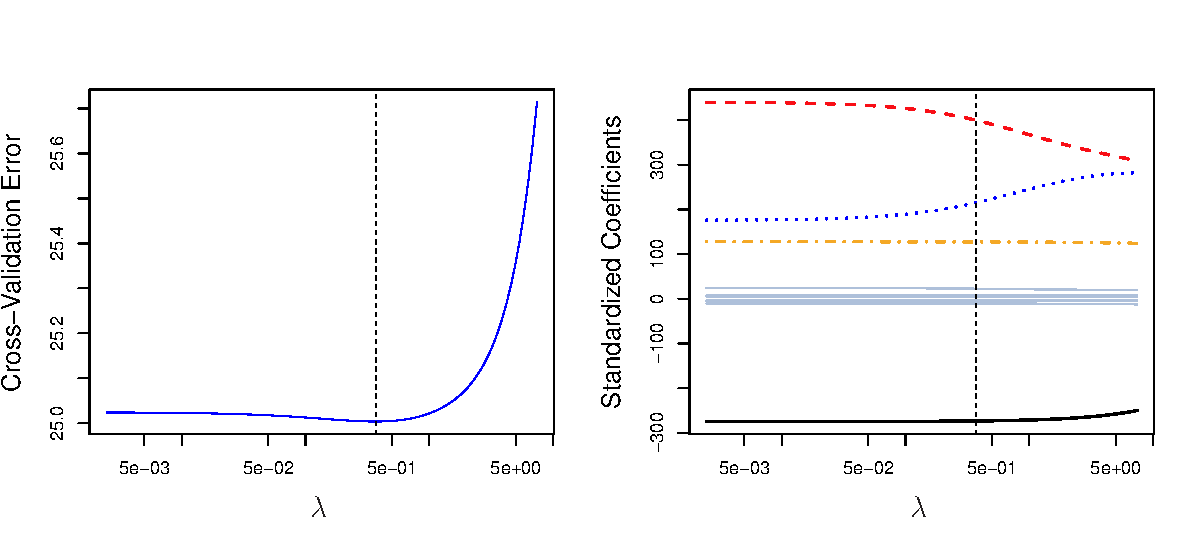
\includegraphics[width=\textwidth]{figures/6_12}
    \vspace{-5mm}
    \begin{itemize}
        \footnotesize
        \item \textbf{Left Panel:} Cross-validation errors that result from applying ridgev regression to the Credit data set with various values of $\lambda$.
        \item \textbf{Right Panel:} The coefficient estimates as a function of $\lambda$. The vertical dashed lines indicates the value of $\lambda$ selected by cross-validation.
    \end{itemize}
\end{frame}

\begin{frame}{Simulated data example}
    \centering
    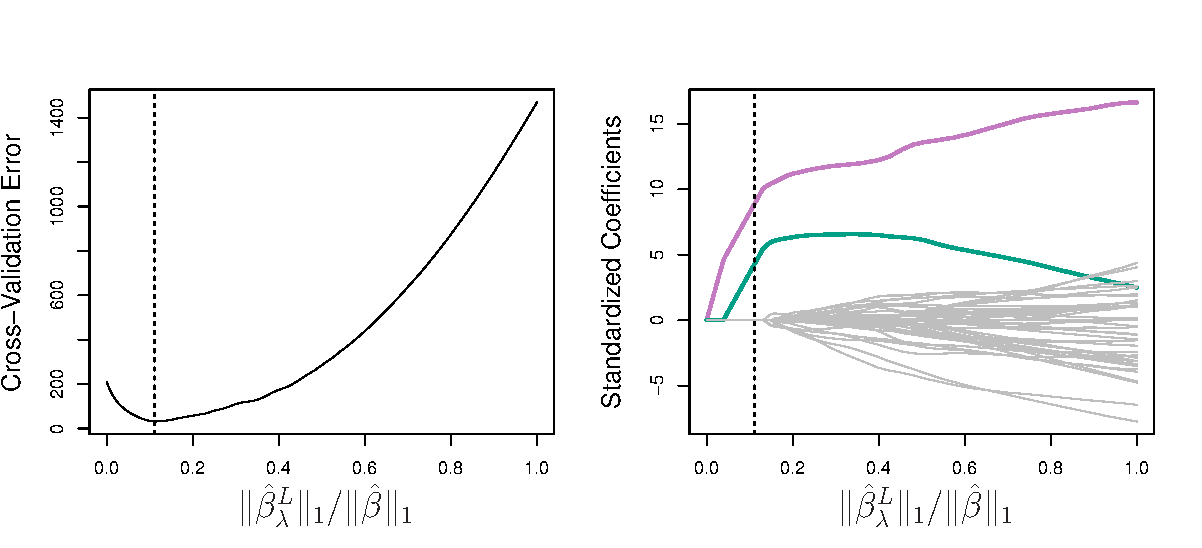
\includegraphics[width=\textwidth]{figures/6_13}
    \vspace{-5mm}
    \begin{itemize}
        \footnotesize
        \item \textbf{Left Panel:} Ten-fold cross-validation \textit{MSE} for the lasso, applied to the sparse simulated data set from Slide 39.
        \item \textbf{Right Panel:} The corresponding lasso coefficient estimates are displayed. The vertical dashed lines indicate the lasso fit for which the cross-validation error is smallest.
    \end{itemize}
\end{frame}

\section{Dimension Reduction Methods}

\begin{frame}{Dimension Reduction Methods}
    \begin{itemize}
        \item Rather than selecting subsets or shrinking original features, \textbf{dimension reduction methods} transform predictors:
        \[
            Z_m = \sum_{j=1}^p \phi_{jm} X_j, \quad m = 1, \dots, M \quad (M < p)
        \]
        \item Then fit an OLS regression model using the $M$ transformed features:
        \[
            y_i = \theta_0 + \sum_{m=1}^M \theta_m z_{im} + \epsilon_i, \quad i = 1, \dots, n
        \]
        \item Notice that $\sum_{m=1}^M \theta_m z_{im} = \sum_{j=1}^p \left(\sum_{m=1}^M \theta_m \phi_{jm}\right) x_{ij} = \sum_{j=1}^p \beta_j x_{ij}$, where $\beta_j = \sum_{m=1}^M \theta_m \phi_{jm}$.
        \item Constrains coefficient vector to an $M$-dimensional subspace, mitigating overfitting.
    \end{itemize}
\end{frame}

\begin{frame}{Principal Components Regression (PCR)}
    \begin{itemize}
        \item \textbf{Principal Components Regression (PCR)} constructs the first $M$ principal components $Z_1, \dots, Z_M$ and uses them as predictors in least squares regression.
        \vspace{0.4em}
        \item \textbf{Key Assumption:} Directions in feature space that capture the greatest variance in $\mathbf{X}$ are also the directions most associated with $Y$.
        \vspace{0.4em}
        \item \textbf{Properties of PCR:}
        \begin{itemize}
            \item PCR is \textbf{unsupervised}: response $Y$ is \emph{not} used to determine components.
            \item PCR is \emph{not} a feature selection method: each $Z_m$ is a linear combination of all $p$ original features.
            \item Always \textbf{standardize predictors} prior to computing principal components.
            \item Tuning parameter $M$ ($1 \le M \le p$) is chosen via cross-validation.
        \end{itemize}
    \end{itemize}
\end{frame}

\begin{frame}{Pictures of PCA}
    \centering
    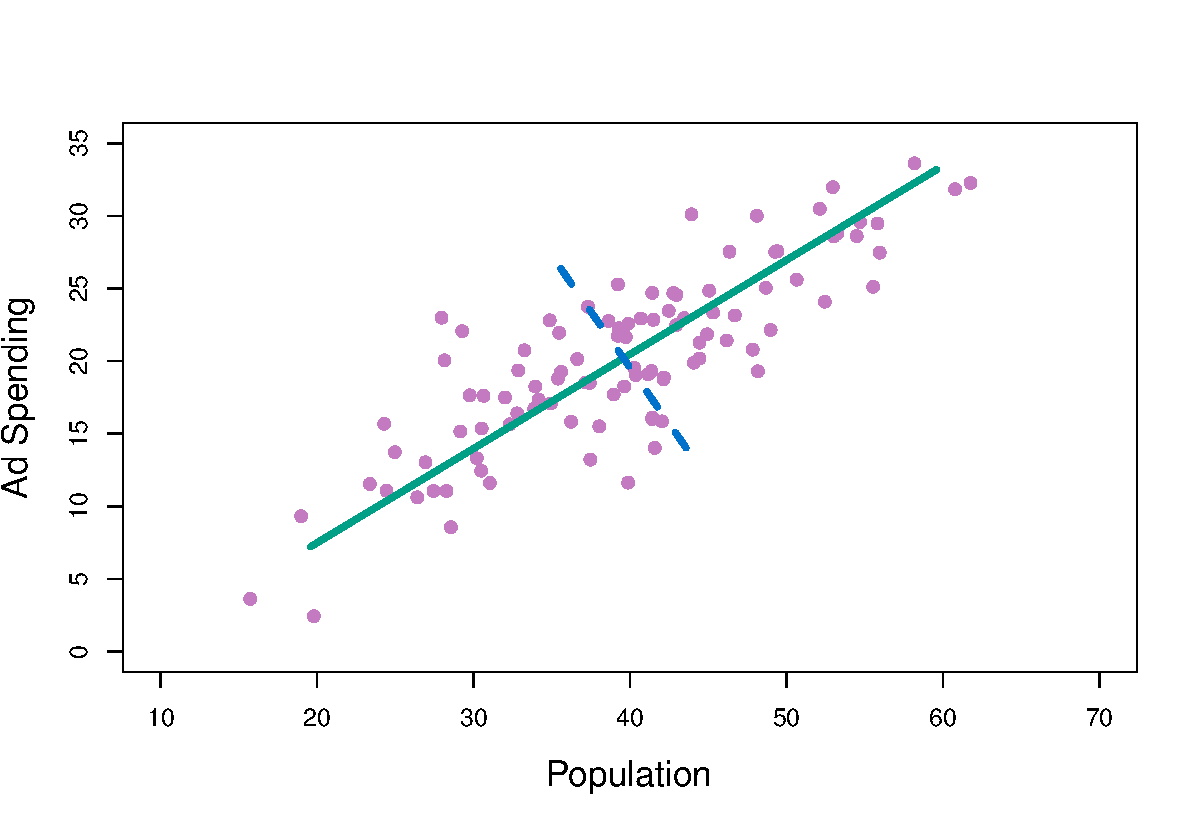
\includegraphics[width=0.75\textwidth]{figures/6_14}
    \begin{itemize}
        \footnotesize
        \item The population size (\texttt{pop}) and ad spending (\texttt{ad}) for 100 different cities are shown as purple circles. The green solid line indicates the first principal component, and the blue dashed line indicates the second principal component.
    \end{itemize}

\end{frame}

\begin{frame}{Pictures of PCA --continued}
    \centering
    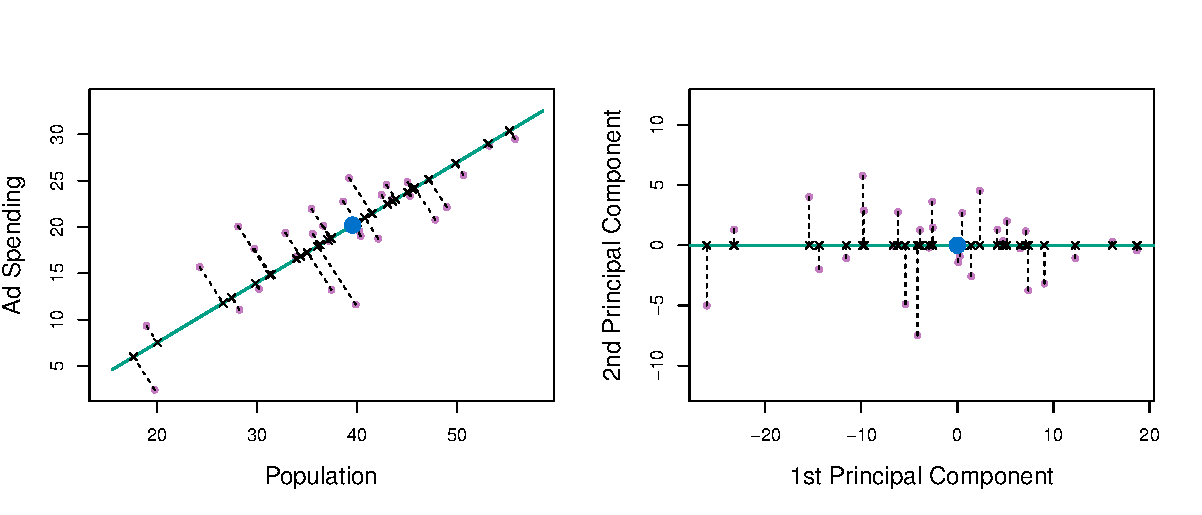
\includegraphics[width=\textwidth]{figures/6_15} \\
    \vspace{-5mm}
    {\tiny A subset of the advertising data.}
    \begin{itemize}
        \footnotesize
        \item \textbf{Left}: The first principal component, chosen to minimize the sum of the squared perpendicular distances to each point, is shown in green. These distances are represented using the black dashed line segments.
        \item \textbf{Right}: The left-hand panel has been rotated so that the first principal component lies on the x-axis.
    \end{itemize}
\end{frame}

\begin{frame}{Pictures of PCA --continued}
    \centering
    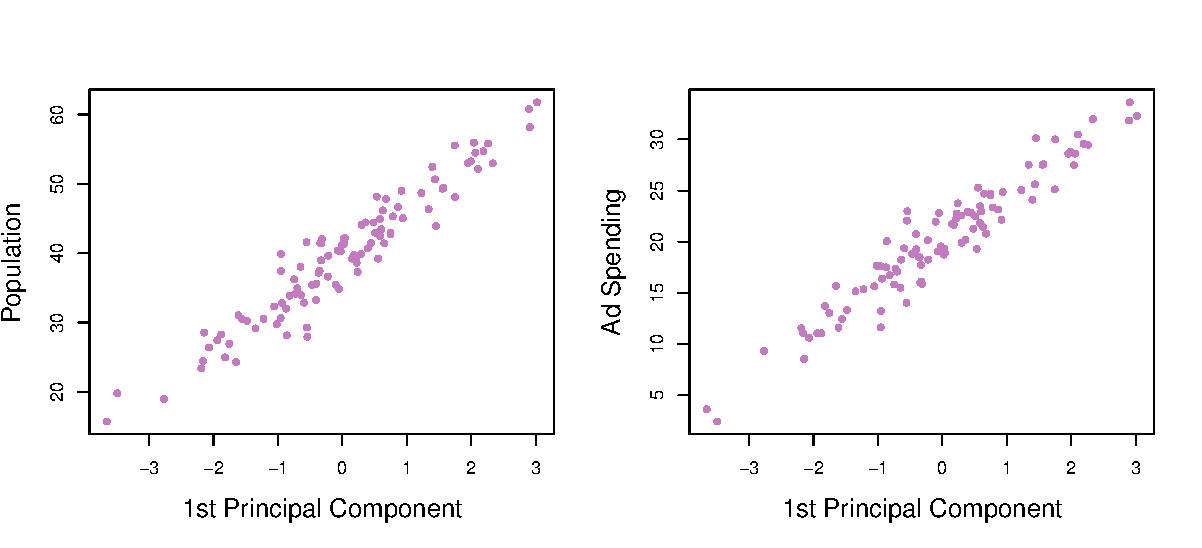
\includegraphics[width=\textwidth]{figures/6_16}
    \begin{itemize}
        \footnotesize
        \item Plots of the first principal component scores $z_{i1}$ versus \texttt{pop} and \texttt{ad}. The relationships are strong.
    \end{itemize}
\end{frame}

\begin{frame}{Pictures of PCA --continued}
    \centering
    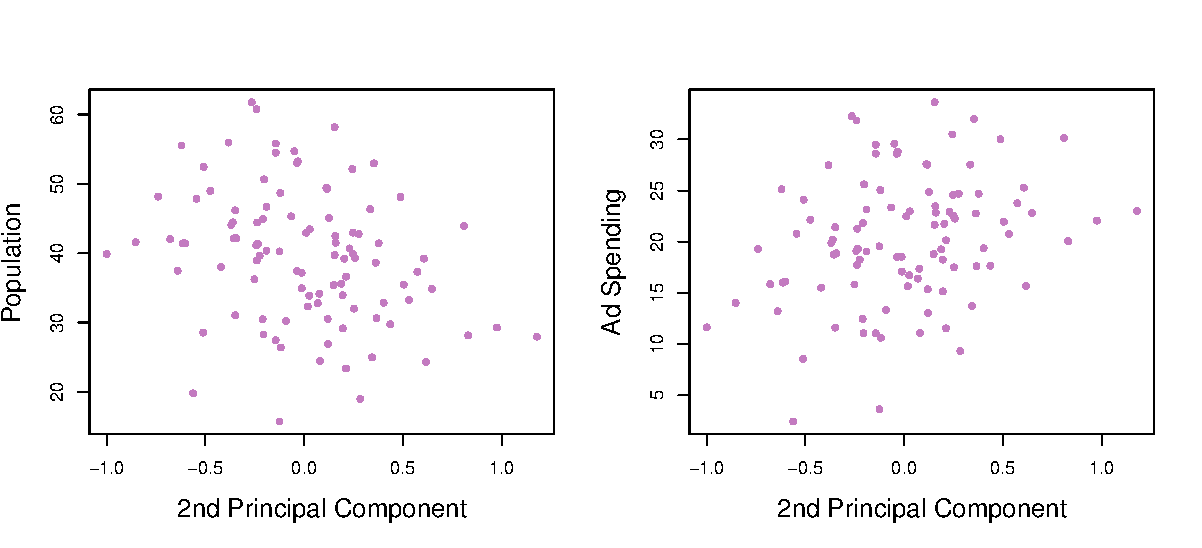
\includegraphics[width=\textwidth]{figures/6_17}
    \begin{itemize}
        \footnotesize
        \item Plots of the second principal component scores $z_{i2}$ versus \texttt{pop} and \texttt{ad}. The relationships are weak.
    \end{itemize}
\end{frame}

\begin{frame}{Application to Principal Components Regression}
    \centering
    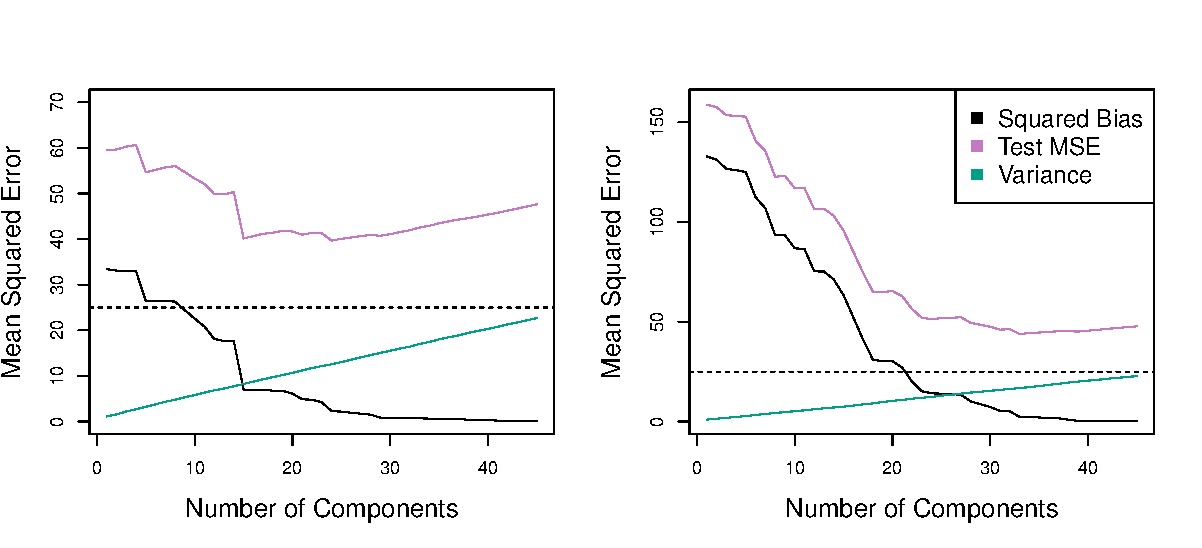
\includegraphics[width=\textwidth]{figures/6_18}
    \vspace{-5mm}
    \begin{itemize}
        \footnotesize
        \item \textit{PCR} was applied to two simulated data sets. The black, green, and purple lines correspond to squared bias, variance, and test mean squared error, respectively.
        \item \textbf{Left}: Simulated data from slide 32.
        \item \textbf{Right}: Simulated data from slide 39.
    \end{itemize}
\end{frame}

\begin{frame}{Choosing the number of directions $M$}
    \centering
    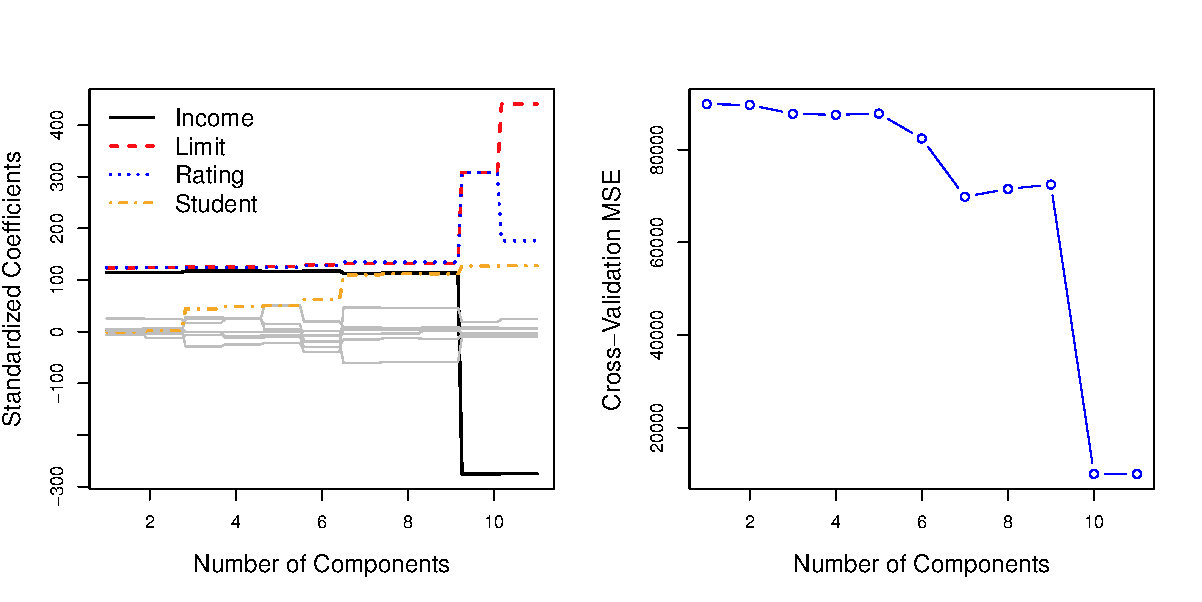
\includegraphics[width=\textwidth]{figures/6_20}
    \vspace{-5mm}
    \begin{itemize}
        \footnotesize
        \item \textbf{Left}: \textit{PCR} standardized coefficient estimates on the \texttt{Credit} data set for different values of $M$.
        \item \textbf{Right}: The 10-fold cross validation \textit{MSE} obtained using \textit{PCR}, as a function of $M$.
    \end{itemize}
\end{frame}

% \begin{frame}{}
%     \centering
%     \includegraphics[width=\textwidth]{}
% \end{frame}

\begin{frame}{Partial Least Squares (PLS)}
    \begin{itemize}
        \item \textbf{Drawback of PCR:} As an unsupervised method, PCA may construct directions with large predictor variance that happen to have zero correlation with $Y$.
        \item \textbf{Partial Least Squares (PLS)} is a \textbf{supervised} dimension reduction technique:
    \end{itemize}
    \begin{block}{Algorithm: Partial Least Squares (First Directions)}
    \begin{enumerate}
        \item Standardize all $p$ predictors and center the response $Y$.
        \item Compute the first direction $Z_1 = \sum_{j=1}^p \phi_{1j} X_j$ by setting $\phi_{1j}$ equal to the slope from regressing $Y$ onto $X_j$ ($\phi_{1j} \propto \text{Cor}(X_j, Y)$).
        \item \textbf{Orthogonalize:} Regress each $X_j$ on $Z_1$ and compute residuals (unexplained variation).
        \item Compute $Z_2$ on these residuals using the same strategy, and repeat for $M$ steps.
        \item Fit multiple linear regression of $Y$ on $Z_1, \dots, Z_M$ via least squares.
    \end{enumerate}
    \end{block}
\end{frame}

\begin{frame}{PLS vs. PCR Comparison}
    \centering
    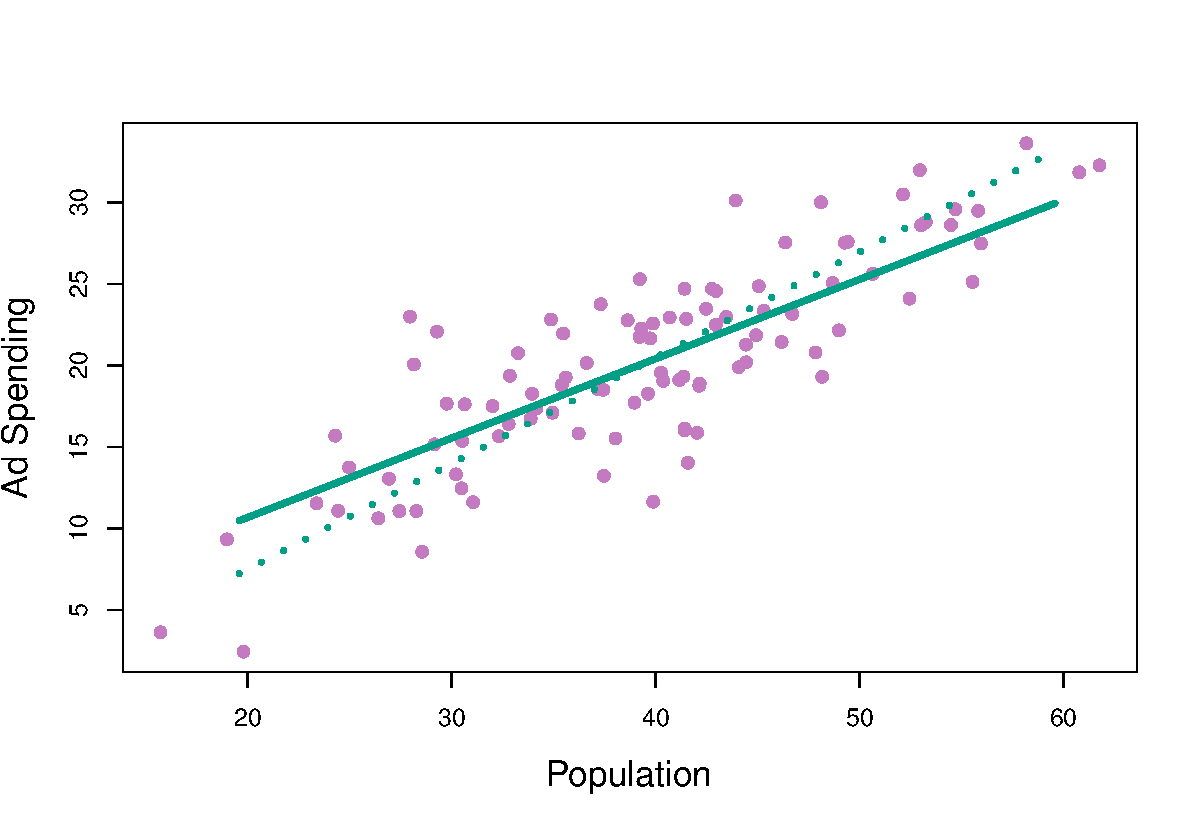
\includegraphics[width=0.7\textwidth]{figures/6_21}
    \begin{itemize}
        \footnotesize
        \item Comparison of first principal component (unsupervised PCR direction, dotted line) and first partial least squares direction (supervised PLS direction, solid line) on advertising data.
        \item PLS tilts the direction toward \texttt{pop} because \texttt{pop} is more strongly correlated with the sales response than \texttt{ad} spending.
    \end{itemize}
\end{frame}

\section{Considerations in High Dimensions}

\begin{frame}{High-Dimensional Data: What Goes Wrong?}
    \begin{itemize}
        \item Modern datasets frequently operate in the \textbf{high-dimensional regime} ($p > n$ or $p \approx n$).
        \item Examples: Genomics (thousands of SNPs, hundreds of patients), text processing, finance.
    \end{itemize}
    \begin{columns}[T]
        \begin{column}{0.48\textwidth}
            \begin{alertblock}{Pitfalls of OLS when $p \ge n$}
                \begin{itemize}
                    \item OLS will fit the training data perfectly ($R^2 = 1$, $\text{RSS} = 0$).
                    \item Infinitely many solutions exist; standard error formulas fail ($\hat{\sigma}^2 = 0$).
                    \item Severe \textbf{overfitting} causes catastrophic test set error.
                \end{itemize}
            \end{alertblock}
        \end{column}

        \begin{column}{0.48\textwidth}
            \begin{alertblock}{Failure of Classical Criteria}
                \begin{itemize}
                    \item $C_p$, AIC, and BIC require estimating $\sigma^2$ from the full model, which is impossible when $p > n$.
                    \item Adjusted $R^2$ easily produces artificial values of 1.
                    \item Regularization or cross-validation is strictly mandatory.
                \end{itemize}
            \end{alertblock}
        \end{column}
    \end{columns}
\end{frame}

\begin{frame}{High Dimensions: Training vs. Test Performance}
    \centering
    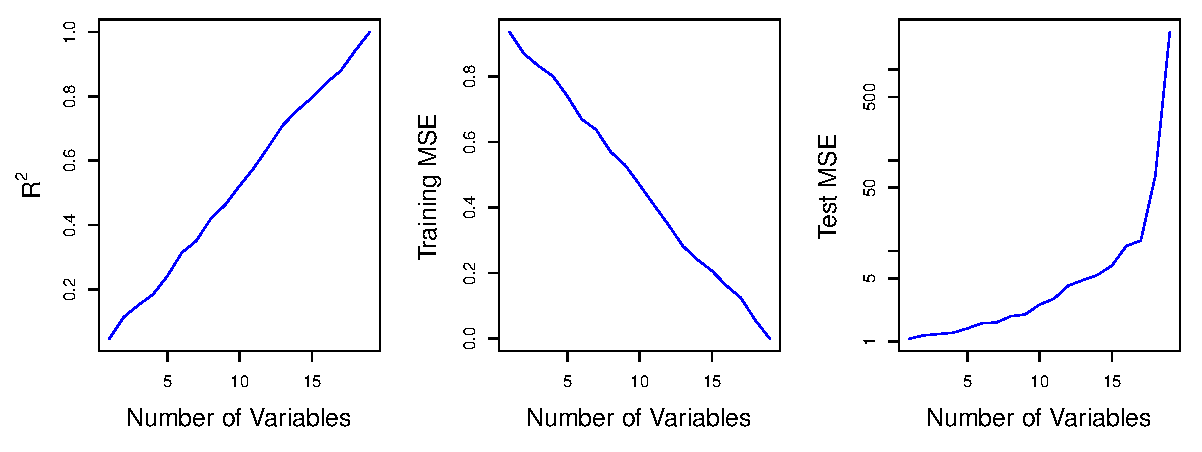
\includegraphics[width=\textwidth]{figures/6_23}
    \vspace{-5mm}
    \begin{itemize}
        \footnotesize
        \item Simulated experiment with fixed sample size $n = 20$ where unrelated noise features are added one by one.
        \item \textbf{Left:} $R^2$ climbs to $1.0$ as $p \to 20$.
        \item \textbf{Center:} Training MSE drops to $0.0$.
        \item \textbf{Right:} Test set MSE explodes as additional noise predictors enter the model.
    \end{itemize}
\end{frame}

\begin{frame}{Interpreting Results in High Dimensions}
    \begin{itemize}
        \item \textbf{Extreme Collinearity:} In high dimensions, any variable can typically be written as an almost exact linear combination of the others.
        \vspace{0.5em}
        \item \textbf{Never Claim "The" True Model:}
        \begin{itemize}
            \item If Lasso or Forward Stepwise selects 15 genes to predict cancer recurrence, it does \emph{not} mean those 15 genes are the only causal drivers.
            \item Other correlated gene sets would achieve nearly identical predictive accuracy.
        \end{itemize}
        \vspace{0.5em}
        \item \textbf{Validation is Mandatory:}
        \begin{itemize}
            \item Never trust training set performance or standard $p$-values after model selection.
            \item Model assessment must be conducted on completely independent test data or through rigorous cross-validation.
        \end{itemize}
    \end{itemize}
\end{frame}

\section{Summary}

\begin{frame}{Summary}
    \begin{table}
        \centering
        \footnotesize
        \begin{tabular}{l l c p{4.75cm}}
            \toprule
            \textbf{Method} & \textbf{Selection Type} & \textbf{Sparsity} & \textbf{Key Strength / When to Use} \\
            \midrule
            \textbf{Best Subset} & Discrete Search & Yes & Optimal for very small $p$ ($p \le 20$). \\
            \addlinespace[0.3em]
            \textbf{Forward Stepwise} & Greedy Search & Yes & Scalable subset method; works when $p > n$. \\
            \addlinespace[0.3em]
            \textbf{Ridge Regression} & $\ell_2$ Shrinkage & No & Superb under multicollinearity \& dense signals. \\
            \addlinespace[0.3em]
            \textbf{The Lasso} & $\ell_1$ Shrinkage & Yes & Produces sparse, interpretable models. \\
            \addlinespace[0.3em]
            \textbf{PCR} & Unsupervised Subspace & No & High collinearity; large predictor variance. \\
            \addlinespace[0.3em]
            \textbf{PLS} & Supervised Subspace & No & High collinearity; supervised direction tuning. \\
            \bottomrule
        \end{tabular}
    \end{table}
\end{frame}

\begin{frame}{Summary}
    \begin{tcolorbox}[colback=blue!5!white,colframe=blue!75!black,title=Core Conclusion]
        No single method uniformly dominates. When the true model is sparse, Lasso and subset selection excel; when many predictors have small, non-zero effects, Ridge regression and PCR often perform best. Tuning parameters ($\lambda, M$) should always be chosen via cross-validation.
    \end{tcolorbox}
\end{frame}

\begin{frame}{}
    \centering
    \Huge End of Chapter 6.
\end{frame}

\begin{frame}{An Introduction to Statistical Learning with Applications in R}{a.k.a. ISLR}
    \centering
    
\includegraphics[height=0.7\textheight]{figures/book_cover} \\
    \vspace{4mm}
    {
        \tiny
        Content has been extracted from \textit{An Introduction to Statistical Learning with Applications in R}, Second Edition, by James, Witten, Hastie \& Tibshirani. Springer. 2023.\\
        Visit \url{https://www.statlearning.com/}.\\
    }
\end{frame}

\end{document}
